%------------------------------------------
% README
%------------------------------------------
% MSc. CAVE latex template
%
% This is a modification of my thesis template, so there may be some things you want to remove.
% Each chapter is in a separate latex file. Those files are included using \input
% You can keep everything in one file by replacing the line "\input{...}" by the content of your chapter 
% Separate files are made so that you can compile chapters independently. Latex can be long to compile large documents
% if your thesis is not too long, then you should probably keep everything in one file.

% I use a lot of margin and padding. Feel free to change it in format-setup. If you have additional package, you can add them in format-setup.
% You can change practically everything in latex, just google it, there are always plenty of answers.


\newcommand{\isEmbedded}{true}


\documentclass[12pt]{report}
	
% FONT RELATED
%\usepackage{times} %Move to times font
\usepackage[labelfont=bf,textfont=it]{caption}
\usepackage[utf8]{inputenc}

% LINKS, PAGE OF CONTENT, REF AND CROSS-REF, HEADERS/FOOTERS
\usepackage[hidelinks]{hyperref}
\usepackage{fancyhdr}
\usepackage{acronym}

% FIGURES, GRAPHICS, TABLES
\usepackage{graphicx}
\usepackage{parskip}
%\usepackage{subfigure}
\usepackage{subfig}
\usepackage{wrapfig}
\usepackage{subfloat}

% COLOURS, TEXT AND FORMATTING
\usepackage{array}
\usepackage{color}
\usepackage{setspace}
\usepackage{longtable}
\usepackage{multirow}

% ADVANCED MATHS, PSEUDO-CODE
\usepackage{amsmath}
\usepackage{alltt}
\usepackage{amsfonts}

% BIBLIOGRAPHY
\usepackage[authoryear]{natbib}
\bibpunct{(}{)}{;}{a}{,}{,}

% USE IN DISSER:

\setlength\oddsidemargin{0.85cm}
\setlength\evensidemargin{0.85cm}

\setlength\textheight{21.0cm}
\setlength\textwidth{15.0cm}

% indent at each new paragrapg
\setlength\parindent{0.5cm}

\setlength\topmargin{-0.2in}
\renewcommand{\baselinestretch}{1.3}

%REPORT

%\setlength\oddsidemargin{1cm}
%\setlength\evensidemargin{0.3in}
%%\setlength\headsep{2.5in}
%
%\setlength\textheight{9.0in}
%\setlength\textwidth{5.5in}
%
%% indent at each new paragrapg
%\setlength\parindent{0.5cm}
%
%%\setlength{\parskip}{10.5ex}
%
%\setlength\topmargin{-0.2in}

%\newcommand{\HRule}{\rule{\linewidth}{0.5mm}}
\newcommand{\HRule}{\rule{\linewidth}{0.0mm}}

% Color definitions (RGB model)
\definecolor{ms-comment}{rgb}{0.1, 0.4, 0.1}
\definecolor{ms-question}{rgb}{0.4, 0.0, 0.0}
\definecolor{ms-new}{rgb}{0.2, 0.4, 0.8}



\begin{document}

% Front page

\begin{titlepage}

\begin{center}

~\\[4.0cm]
{ \huge \bfseries Crowd Simulation}\\[0.5cm]
{ \Large \bfseries based on emergent behaviours}\\[1.0cm]

{\large
\textsc{Carlos Pérez López}\\[1.5cm]


{\large August, 2013}\\[3.5cm]

%A thesis submitted in partial fulfilment of the requirements of Bournemouth University for the degree of Doctor of Philosophy
%\\[2.0cm]

\textbf{Master of Science,}\\[0.25cm]
\textbf{Computer Animation and Visual Effects}\\[1.0cm]
%\textbf{}\\[0.5cm]


\includegraphics[width=0.3\textwidth]{img/bu_logo}\\[1cm]

}

\vfill

\end{center}

\end{titlepage}



\section*{}

\begin{itshape}

%\centering
In memory of my grandpa:\\

My grandpa used to wear a blue jacket. I have not ever asked where he bought it, but I assume he took it in the  cloth shop he built from scratch, and called with his wife's name.

My grandpa used to give hidden tip to the bartender to get extra olives for his grandchildren, while he pretended to look at his wine.

Lately, my grandpa used to forget things, that is why my grandma received birthday's cakes several times a year (none of them in the right date).

My grandpa was sometimes very grumpy, but his smile warmed more than the Sun.

My grandpa always gave me the money for the bus when I left on Sundays, even when I left to other country with an Erasmus scholarship.

My grandpa agreed to my mother that buying me a car could be dangerous, but he gave me driving lessons on Fridays' afternoon.

When I was younger, I was always crying because I did not want to attend to a piano lesson with a very tough teacher, but suddenly one day she was lovely; later I discovered she had met my grandpa.

My grandpa used to build kites with old papers from the cloth shop, pasting them to wooden sticks with hot potato. One day he put a kite higher than the clouds. Other day he arose from a sea of spiny plants with a lost kite on his hand shouting: "I won't fly it again!". But he did.

My grandpa once caught a falcon.

When I was young, my grandpa told me that some turtles used to stay very quiet for a long time. After discovering that my turtle died, I knew that my grandpa had gone hidden to the pet shop to try to buy another one, but they did not have more.

When I got older, my grandpa always reminded me to carry socks to excursions; not the ones which come in pairs, but the ones which come in boxes of six or twelve.

Every night my grandpa gave me a cup of chamomile. Once, I threw it with my elbow and he shouted at me, and I ran to my bed crying. I do not remember how much time later, but it was exactly the time chamomile requires to be done, because there he was, waking me up, grabbing a cup with both hands.

Girls called me many things, even tons of them did not ever call me at all. But once, one said to me that I was authentic. My grandpa was authentic, genuine. He was a real person, a real human being.

My grandpa taught me the value of a good heart, a sharp mind and big nuts.

\end{itshape}

% Copyrights
\setcounter{page}{1}
\pagenumbering{roman}

% You dont need copyright declaration for your thesis
%
\section*{Copyright statement}
%\addcontentsline{toc}{section}{Copyright statement}
\label{sec:copyrights}
This copy of the thesis has been supplied on condition that anyone who consults it is understood to recognise that its copyright rests with its author and due acknowledgement must always be made of the use of any material contained in, or derived from, this thesis.
%\pagebreak

% Table of contents, figures and tables.
% You NEED a table of contents
\addcontentsline{toc}{section}{Table of contents}
\tableofcontents
\pagebreak
% You can comment out list of figures and tables, it could be too much
%\addcontentsline{toc}{section}{List of figures}
%\listoffigures
%\pagebreak
% You can comment out list of figures and tables, it could be too much
%\addcontentsline{toc}{section}{List of tables}
%\listoftables
%\pagebreak
% No need for abbreviations, but if you use any, define them first (e.g.: We use parametric surfaces such as Non-uniform rational B-spline (NURBS). NURBS are defined by...)
%
\section*{List of Acronyms}
\addcontentsline{toc}{section}{List of Acronyms}

\begin{acronym}[NURBS ]
\acro{ADF}{Adaptively sampled Distance Field}
\acro{BRep}{Boundary representation}
\acro{CAD}{Computer-Aided Design}
\acro{CSG}{Constructive Solid Geometry}
\acro{FRep}{Function representation}
\acro{MVC}{Mean Value Coordinates}
\acro{NURBS}{Non-uniform rational B-Spline}
\acro{SDF}{Signed distance field}
\acro{STTI}{Space Time Transfinite Interpolation}
\acro{TI}{Transfinite Interpolation}
\end{acronym}

\pagebreak
%\pagebreak

\graphicspath{{./img/}}

% Abstract

\ifx\isEmbedded\undefined

\documentclass[12pt]{report}
	
% FONT RELATED
%\usepackage{times} %Move to times font
\usepackage[labelfont=bf,textfont=it]{caption}
\usepackage[utf8]{inputenc}

% LINKS, PAGE OF CONTENT, REF AND CROSS-REF, HEADERS/FOOTERS
\usepackage[hidelinks]{hyperref}
\usepackage{fancyhdr}
\usepackage{acronym}

% FIGURES, GRAPHICS, TABLES
\usepackage{graphicx}
\usepackage{parskip}
%\usepackage{subfigure}
\usepackage{subfig}
\usepackage{wrapfig}
\usepackage{subfloat}

% COLOURS, TEXT AND FORMATTING
\usepackage{array}
\usepackage{color}
\usepackage{setspace}
\usepackage{longtable}
\usepackage{multirow}

% ADVANCED MATHS, PSEUDO-CODE
\usepackage{amsmath}
\usepackage{alltt}
\usepackage{amsfonts}

% BIBLIOGRAPHY
\usepackage[authoryear]{natbib}
\bibpunct{(}{)}{;}{a}{,}{,}

% USE IN DISSER:

\setlength\oddsidemargin{0.85cm}
\setlength\evensidemargin{0.85cm}

\setlength\textheight{21.0cm}
\setlength\textwidth{15.0cm}

% indent at each new paragrapg
\setlength\parindent{0.5cm}

\setlength\topmargin{-0.2in}
\renewcommand{\baselinestretch}{1.3}

%REPORT

%\setlength\oddsidemargin{1cm}
%\setlength\evensidemargin{0.3in}
%%\setlength\headsep{2.5in}
%
%\setlength\textheight{9.0in}
%\setlength\textwidth{5.5in}
%
%% indent at each new paragrapg
%\setlength\parindent{0.5cm}
%
%%\setlength{\parskip}{10.5ex}
%
%\setlength\topmargin{-0.2in}

%\newcommand{\HRule}{\rule{\linewidth}{0.5mm}}
\newcommand{\HRule}{\rule{\linewidth}{0.0mm}}

% Color definitions (RGB model)
\definecolor{ms-comment}{rgb}{0.1, 0.4, 0.1}
\definecolor{ms-question}{rgb}{0.4, 0.0, 0.0}
\definecolor{ms-new}{rgb}{0.2, 0.4, 0.8}


\begin{document}
%\maketitle
\fi

% The begin{abstract} seems to bug the page counter
\section*{Abstract}
\addcontentsline{toc}{section}{Abstract}
\label{sec:abstract}
%\begin{abstract}

{
The use of crowds in films and games requires time and money, either hiring extra cast or animating 3D characters by keyframing. This thesis presents an approach to simulate crowds employing an agent-based model. Although many researches have been done in this field, the method proposed here has significant differences which enhance flexibility and scalability and achieve realistic results. The simulation is entirely driven by the individual script-based behaviours. In this way, the group behaviour of the crowd will emerge from the individuals; from how they interact with each other and with the environment. Hence, very complex simulations can arise from simple behaviours.
}

%\end{abstract}


\ifx\isEmbedded\undefined
% References
\addcontentsline{toc}{chapter}{References}
\bibliographystyle{ref/harvard}
\bibliography{ref/master}
\pagebreak
\end{document}
\fi
\pagebreak
% Acknoedledgements
\section*{Acknowledgements}
\addcontentsline{toc}{section}{Acknowledgements}

To my parents, who paid the bills.

\pagebreak

% Declaration -> Dont include it, unless you have something important to put in there. 
%
\section*{Declaration}
\addcontentsline{toc}{section}{Declaration}

This thesis has been created by myself and has not been submitted in any previous application for any degree. The work in this thesis has been undertaken by myself except where otherwise stated.
%The materials related to hybrid modelling technique based on 
%PUT YOUR PUBLICATIONS HERE

\pagebreak

\setcounter{page}{1}
\pagenumbering{arabic}
% Chapters

\ifx\isEmbedded\undefined

\documentclass[12pt]{report}
	
% FONT RELATED
%\usepackage{times} %Move to times font
\usepackage[labelfont=bf,textfont=it]{caption}
\usepackage[utf8]{inputenc}

% LINKS, PAGE OF CONTENT, REF AND CROSS-REF, HEADERS/FOOTERS
\usepackage[hidelinks]{hyperref}
\usepackage{fancyhdr}
\usepackage{acronym}

% FIGURES, GRAPHICS, TABLES
\usepackage{graphicx}
\usepackage{parskip}
%\usepackage{subfigure}
\usepackage{subfig}
\usepackage{wrapfig}
\usepackage{subfloat}

% COLOURS, TEXT AND FORMATTING
\usepackage{array}
\usepackage{color}
\usepackage{setspace}
\usepackage{longtable}
\usepackage{multirow}

% ADVANCED MATHS, PSEUDO-CODE
\usepackage{amsmath}
\usepackage{alltt}
\usepackage{amsfonts}

% BIBLIOGRAPHY
\usepackage[authoryear]{natbib}
\bibpunct{(}{)}{;}{a}{,}{,}

% USE IN DISSER:

\setlength\oddsidemargin{0.85cm}
\setlength\evensidemargin{0.85cm}

\setlength\textheight{21.0cm}
\setlength\textwidth{15.0cm}

% indent at each new paragrapg
\setlength\parindent{0.5cm}

\setlength\topmargin{-0.2in}
\renewcommand{\baselinestretch}{1.3}

%REPORT

%\setlength\oddsidemargin{1cm}
%\setlength\evensidemargin{0.3in}
%%\setlength\headsep{2.5in}
%
%\setlength\textheight{9.0in}
%\setlength\textwidth{5.5in}
%
%% indent at each new paragrapg
%\setlength\parindent{0.5cm}
%
%%\setlength{\parskip}{10.5ex}
%
%\setlength\topmargin{-0.2in}

%\newcommand{\HRule}{\rule{\linewidth}{0.5mm}}
\newcommand{\HRule}{\rule{\linewidth}{0.0mm}}

% Color definitions (RGB model)
\definecolor{ms-comment}{rgb}{0.1, 0.4, 0.1}
\definecolor{ms-question}{rgb}{0.4, 0.0, 0.0}
\definecolor{ms-new}{rgb}{0.2, 0.4, 0.8}


\graphicspath{{../img/}}
\begin{document}
%\maketitle
\fi

\chapter{Introduction}
\label{chap:intro}

Currently, the presence of crowds in visual pieces, let they be films or video games, has acquired a lot of relevance. Scenes with a crowded train station, big streets full of pedestrians, tons of animals in a flock, troops of robots, hordes of zombies or armies of warriors can be found very often in modern films and games.

In the past, not many films could afford this kind of resources in their scenes, since the only way of having more characters was actually including more characters in the cast. The use of extras highly increases the cost of a production, besides the requirement of a strict coordination and proper training in some situations. One of the reasons of the boom of big masses in films was the arrival of new technologies in computer graphics and artificial intelligence. Alongside with this, the generation and simulation of virtual crowds became a reality, saving money and time and making the use of crowds affordable to big and small studios.

Other of the reasons of the popularity of big groups of individuals featured in films is the strength they give to a shot. It is not only a matter of fact that crowds are visually stunning and their magnificence captures the attention of the audience, but also they are powerful tools to tell and enrich a story. At this point of time, it could be hard, if not impossible, to imagine the saga of the Lord of the Rings without those epic battles of tens of thousands of warriors, or imagine the breathtaking apocalyptic scenes without those milliards of zombies wandering around.

Closely tied to the idea of crowd simulation, the concept of behaviour appears. This is what gives life to the crowd and makes the spectator perceive the group nature of it. An army of brave warriors in a battlefield will find enemies and will show aggressive movements; on the other hand, on a ballroom gentlemen and ladies will dance graciously.

\begin{figure}[!h]
  \centering
  \begin{tabular}{c c}
  	\subfloat[Crowd in a train station]{\label{fig:f1}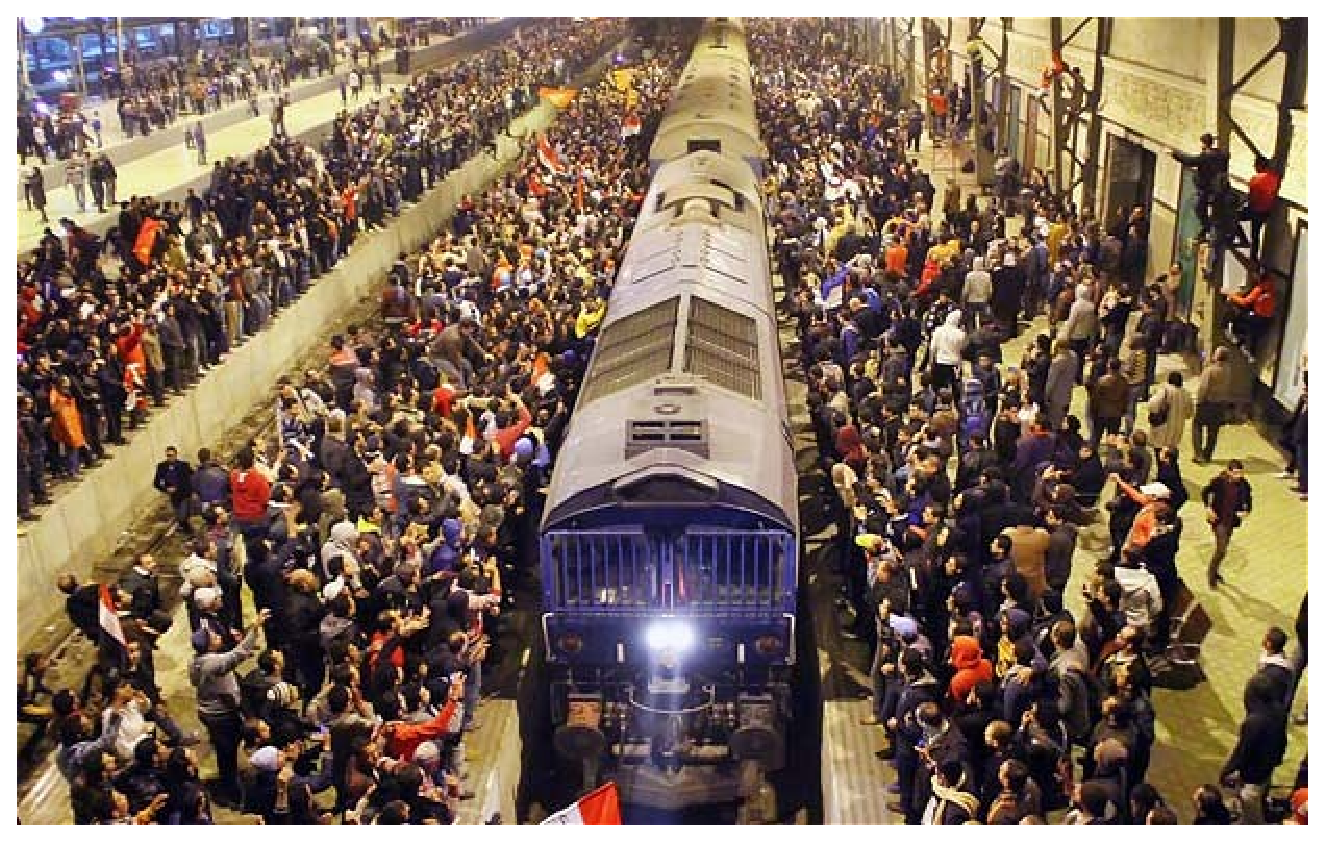
\includegraphics[scale=0.25]{crowd_train.eps}} &
 	\subfloat[Troops of droids (Star Wars)]{\label{fig:f2}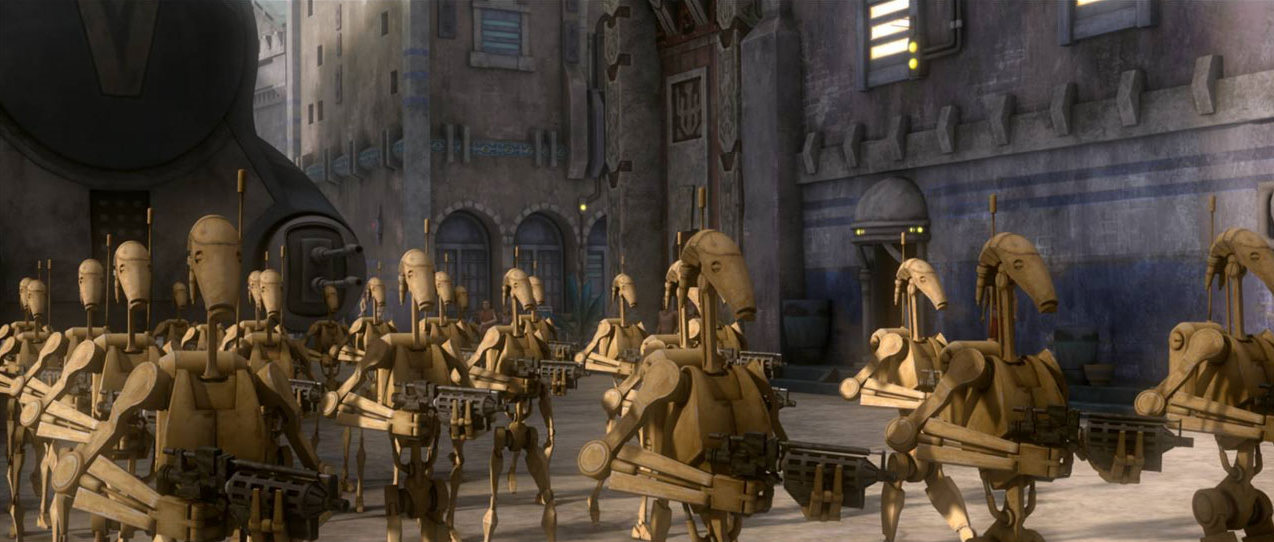
\includegraphics[scale=0.18]{droids.eps}} \\
  	\subfloat[Horde of zombies (World War Z)]{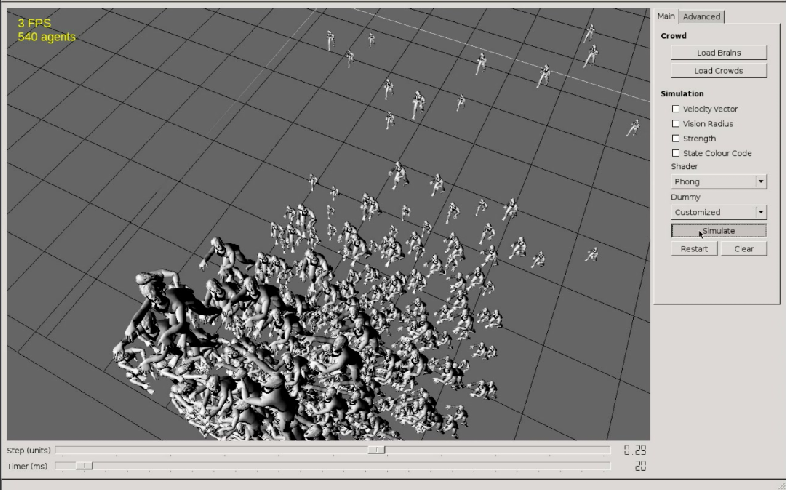
\includegraphics[scale=0.1]{zombies.eps}} & 
  	\subfloat[A Battlefield (Lord of the Rings))]{
\includegraphics[scale=1.5]{battlefield.eps}} \\
  	\subfloat[A Ballroom]{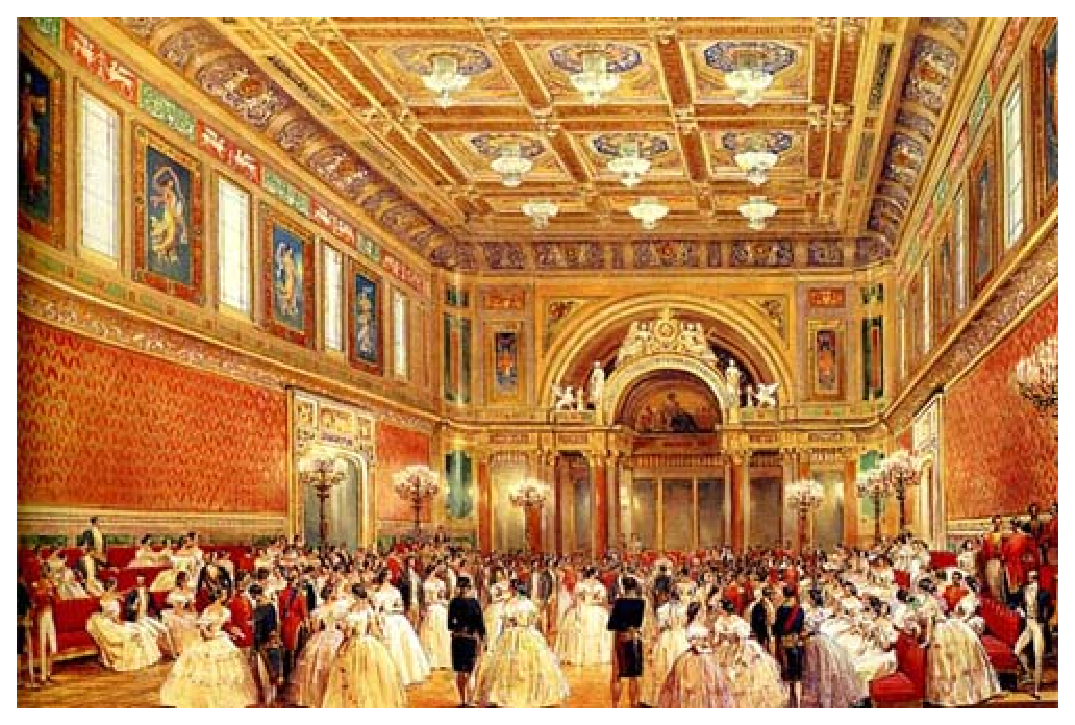
\includegraphics[scale=0.3]{ballroom.eps}} & 
  	\subfloat[One vs Many (Matrix)]{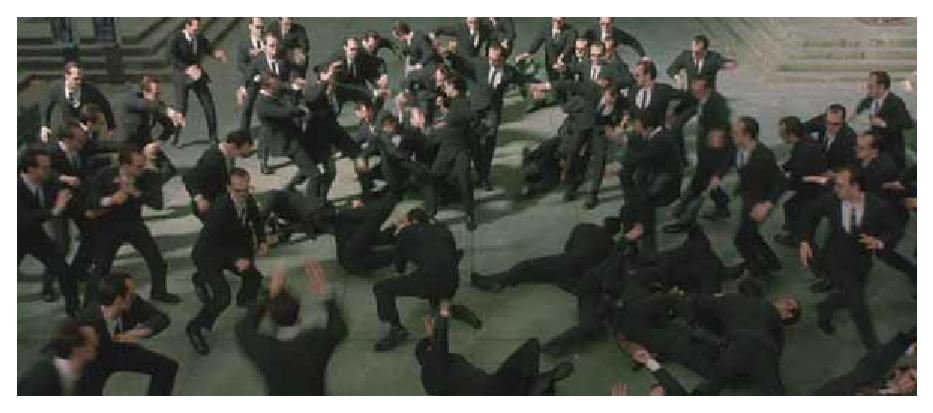
\includegraphics[scale=0.55]{matrix.eps}} \\
 \end{tabular}
  \caption{Crowd scenes}
  \label{fig:crowds}
\end{figure}

The aim of this project is to propose an approach which gives the flexibility to simulate any sort of crowd needed for a scene. Taking base on how the real world works, this method is based on the principle that the group behaviour is determined by the specific behaviours of every individual. And here is where one of the main ideas for this project appears: Emergent Behaviour.

Leonard Kleinrock, professor of computer science in UCLA, states that emergent behaviour is unanticipated behaviour shown by a system \citep{kleinrock}. Once a system is designed and defined by certain rules or mathematical equations, it may configure itself in a way that could not be anticipated. The interaction of a large number of simple individual things is very hard to predict; the complexity does not reside in the individuals, but on the way they are interconnected and they interact to each other. Professor Kleinrock proposes this example: ``we might know how a bunch of children behave when they are alone, but once you put them together in a group, you will observe behaviours that will surprise you''.

Subsequently, how a real crowd behaves is something hard to predict, and how realistic it is depends directly on how realistic each individual is.

This thesis is structured as follows:

\begin{itemize}

\item {{\bf Chapter 2: Related Work.} It explains the previous approaches in this field, the similarities and differences to the proposed method, as well as the advantages and drawbacks they present.}

\item {{\bf Chapter 3: Technical Background.} Physical concepts, flocking algorithms and the force-based virtual world model; and state machines and how they can be used to model behaviours.}

\item {{\bf Chapter 4: Agent Based Model.} This is where the current method starts to be explained into details, using a bottom-up approach. This chapter presents how agents are modeled, the parts which form them and their properties, as well as how they communicate to each other.}

\item{{\bf Chapter 5: Crowd Engine.} Here the core of the approach is introduced. It is explained how to handle the agents efficiently, how the virtual world is designed employing a physically-based approach, and how messages and collisions are faced.}

\item {{\bf Chapter 6: Applications and results.} A pipeline where this methodology might fit in a real production situation is presented. Some results of different tests will be shown in this chapter; a set of individual behaviours will be presented and the emergent behaviour observed will be explained and discussed.}

\item{{\bf Chapter 7: Application design and implementation.} The design and implementation for the application based on this approach are exposed.}

\item {{\bf Chapter 8: Conclusion.} A final concluding chapter will summarize the whole approach, mentioning the main advantages and drawbacks, as well as presenting potential lines for future work.}

\end{itemize}

\ifx\isEmbedded\undefined
% References
\addcontentsline{toc}{chapter}{References}
\bibliographystyle{../ref/harvard}
\bibliography{../ref/master}
\pagebreak
\end{document}
\fi


\ifx\isEmbedded\undefined

\documentclass[12pt]{report}
	
% FONT RELATED
%\usepackage{times} %Move to times font
\usepackage[labelfont=bf,textfont=it]{caption}
\usepackage[utf8]{inputenc}

% LINKS, PAGE OF CONTENT, REF AND CROSS-REF, HEADERS/FOOTERS
\usepackage[hidelinks]{hyperref}
\usepackage{fancyhdr}
\usepackage{acronym}

% FIGURES, GRAPHICS, TABLES
\usepackage{graphicx}
\usepackage{parskip}
%\usepackage{subfigure}
\usepackage{subfig}
\usepackage{wrapfig}
\usepackage{subfloat}

% COLOURS, TEXT AND FORMATTING
\usepackage{array}
\usepackage{color}
\usepackage{setspace}
\usepackage{longtable}
\usepackage{multirow}

% ADVANCED MATHS, PSEUDO-CODE
\usepackage{amsmath}
\usepackage{alltt}
\usepackage{amsfonts}

% BIBLIOGRAPHY
\usepackage[authoryear]{natbib}
\bibpunct{(}{)}{;}{a}{,}{,}

% USE IN DISSER:

\setlength\oddsidemargin{0.85cm}
\setlength\evensidemargin{0.85cm}

\setlength\textheight{21.0cm}
\setlength\textwidth{15.0cm}

% indent at each new paragrapg
\setlength\parindent{0.5cm}

\setlength\topmargin{-0.2in}
\renewcommand{\baselinestretch}{1.3}

%REPORT

%\setlength\oddsidemargin{1cm}
%\setlength\evensidemargin{0.3in}
%%\setlength\headsep{2.5in}
%
%\setlength\textheight{9.0in}
%\setlength\textwidth{5.5in}
%
%% indent at each new paragrapg
%\setlength\parindent{0.5cm}
%
%%\setlength{\parskip}{10.5ex}
%
%\setlength\topmargin{-0.2in}

%\newcommand{\HRule}{\rule{\linewidth}{0.5mm}}
\newcommand{\HRule}{\rule{\linewidth}{0.0mm}}

% Color definitions (RGB model)
\definecolor{ms-comment}{rgb}{0.1, 0.4, 0.1}
\definecolor{ms-question}{rgb}{0.4, 0.0, 0.0}
\definecolor{ms-new}{rgb}{0.2, 0.4, 0.8}


\graphicspath{{../img/}}
\begin{document}
\fi

\chapter{Related work}
\label{chap:related}

Generating crowds is a problem that has frequently been faced in the field of computer graphics and artificial intelligence. Numerous solutions have been proposed, following different approaches and applying different ideas and concepts. Crowd motions can be created by planning or simulation, and even some researches propose hybrid approaches.

\section{Motion Planning for Crowd}

Opposite to the philosophy of this thesis, a substantial sum of research establishes that a crowd is not only a group of individuals and involves problems that should be handled at the group level, making use of pre-planned techniques. Frequently, strategies such as virtual force fields, navigation fields, motion planning, navigation graphs, etc. are employed to drive the movement of the whole mass, forgetting by all means the individual nature of the crowd. S. Musse et al. state that a motion planning for a group walking together requires more information than an individual motion planning \citep{musse1}. In addition, this research claims for the need of model behaviours at the level of groups and crowds in order to acquire the beauty of synchronization, homogeneity and unity.

\begin{figure}[!htb]
  \centering
  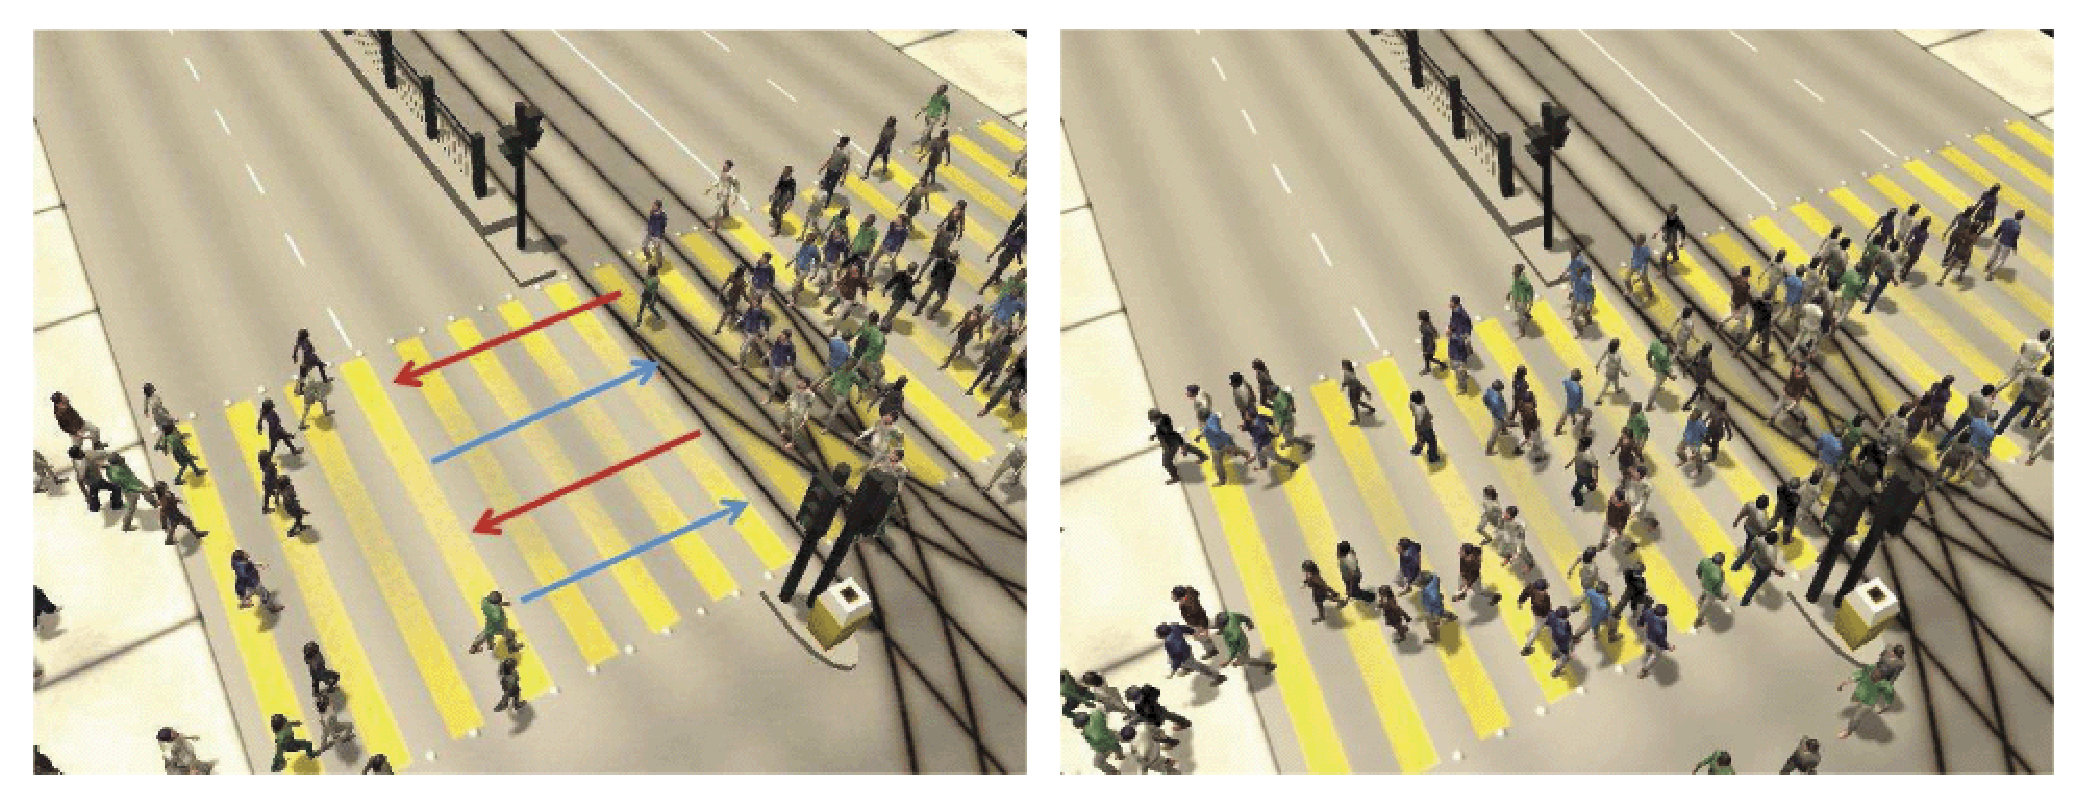
\includegraphics[scale=0.4]{navigation_fields.eps}
  \caption[Motion Planning for Crowd]{Motion Planning for Crowd using Navigation Fields \citep{patil}}
  \label{fig:navigation}
\end{figure}

Extending the control vertically, in \citep{musse2} a hierarchical model for real time simulation of virtual human crowds is proposed allowing different control features at levels of crowd, groups or individuals. This is an example of hybrid approach where it is possible to increase the complexity of crowd-group-individual behaviours according to the problem to be simulated.

By means of these techniques, it was visually proven that very convincing and realistic results can be produced. Nevertheless, the identity and the decision capacity of each of the individuals is partially if not completely lost.

\section{Crowd Motion Simulation}

Purely simulation strategies, which is the case of this thesis, discard any pre-planned decision and the final result is entirely based on the global consequences of local interactions of members of the population. This is known as Agent-Based Model or Individual-Based Model. It will be detailed in Chapter \ref{chap:agent-based_model} and for further information check  \citep{red3D}.

The main idea this thesis is settled on is the simple principle stated by C. Reynolds, the pioneer of flocking behaviours, which claimed that very simple rules can arise emergent behaviours without involving any central coordination. Notice again the concept of emerge.

One of the earliest works  in group behaviours was Craig Reynolds' flocking algorithm which was a distributed behaviour model for flocks, herds and schools \citep{reynolds}. The individuals of his flocking system are called ``Boids'' and are subjected to three simple rules: cohesion, alignment and separation.

This classic research not only presents a flocking algorithm, but also establishes a turning point proposing an individual virtual force model as the way to affect how each agent move. The approach presented in this thesis has adopted that model.

\begin{figure}[!htb]
  \centering
  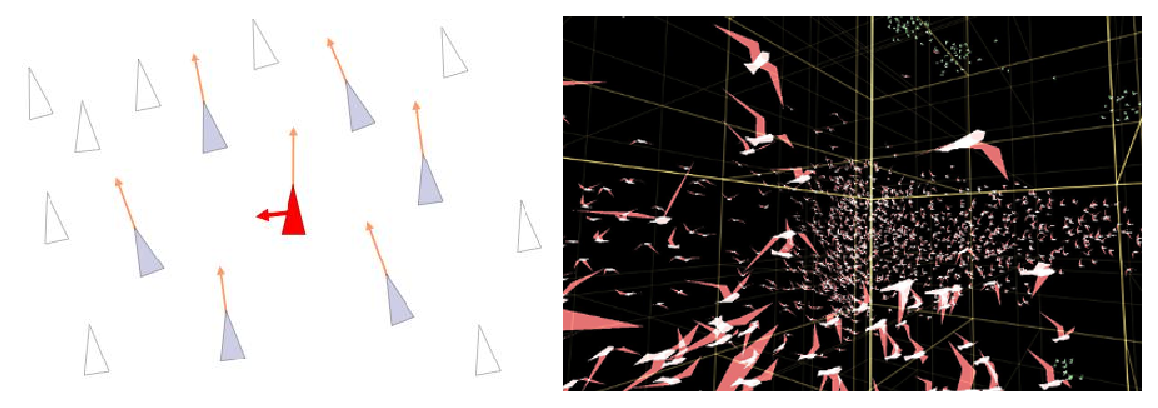
\includegraphics[scale=0.65]{reynolds_flocking.eps}
  \caption[Flocking System]{Flocking System following the Virtual Force Model proposed by C. W. Reynolds \citep{reynolds}}
  \label{fig:massive}
\end{figure}

Starting from this robust and solid idea, tons of research paths can be taken in order to acquire and compare different approaches for crowd simulation. For instance, C. Wang \& T. Li suggest an evolving crowd motion simulation \citep{wang}. In that research, the use of genetic algorithms is proposed to generate optimal virtual forces according to the given environment and desired movement behaviour.

Although Craig Reynolds presents a base-approach which models very accurately the way crowds behave in the real world, the main disadvantage is that configuring the forces to generate desired motion behaviours remains empirical. And again, we are witnesses of a characteristic inherent to emergent behaviours.

\section{MASSIVE Software}

MASSIVE stands for Multiple Agent Simulation System in Virtual Environment and is a software developed by Stephen Regelous in Weta Digital, as a request from Peter Jackson to recreate those epic battle scenes that Tolkien described in the books of the Lord of the Rings. Massive has contributed to the creation of many awarding visual effects, particularly  the battle sequences; and due to this, it has been developed into a complete product and has been licensed by many other visual effects houses.

\begin{figure}[!htb]
  \centering
  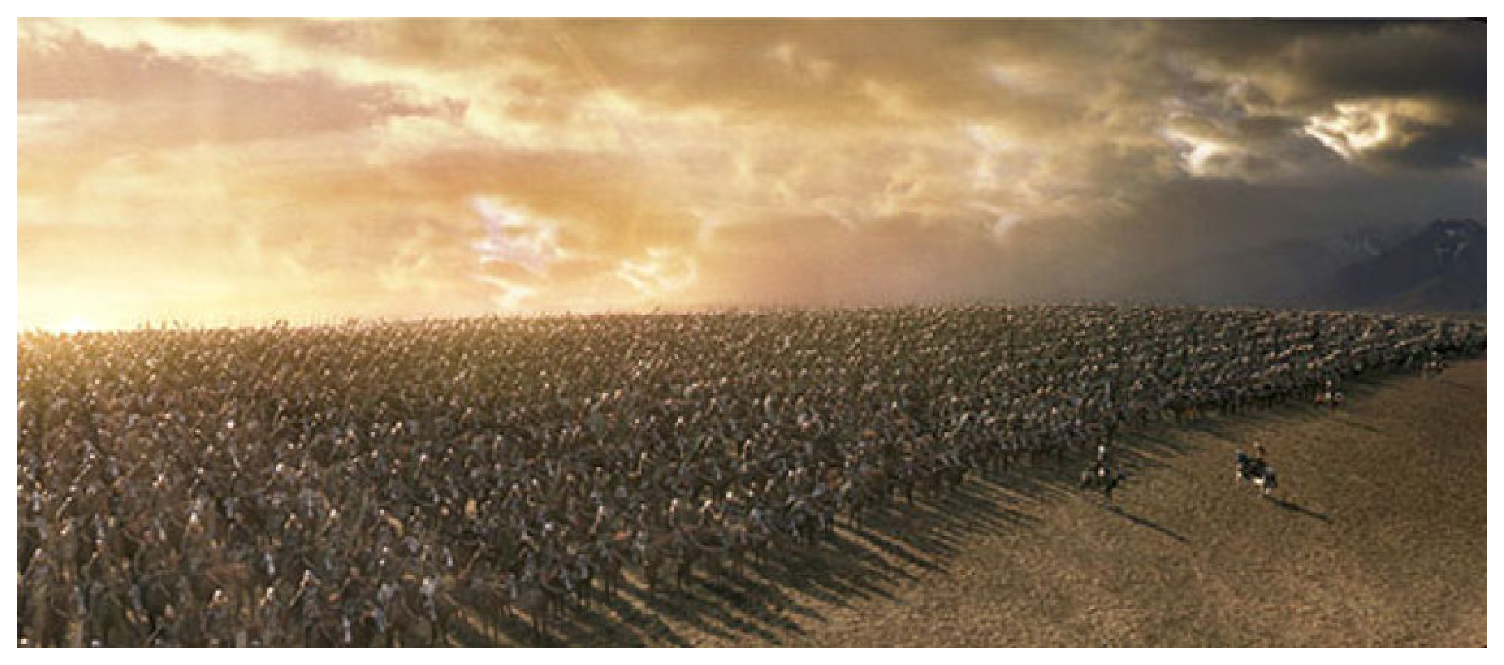
\includegraphics[scale=0.5]{rohan_army.eps}
  \caption[Massive Software]{Award winning battle scene from 'The Lord of the Rings: Return of the King'}
  \label{fig:massive}
\end{figure}

Massive introduces a very interesting model approach which consists of treating each agent as a combination of a body and a brain. The body defines the physical characteristics of the agent and the brain is a fuzzy logic network which controls the actions of the agent such as following an arbitrary terrain, avoiding obstacles or interacting with other agents. This thesis has adopted this natural design combined with the flexibility that scripting languages provide.

Each action is associated to a pre-recorded animation, rather obtained from motion captured session or hand-animated, and will be blended between them in order to achieve the movement of the character. Apart from Artificial Intelligence features, it includes other abilities such as Rigid Body Dynamics (RBD), cloth simulation or GPU rendering. 



\ifx\isEmbedded\undefined
% References
\addcontentsline{toc}{chapter}{References}
\bibliographystyle{../ref/harvard}
\bibliography{../ref/master}
\pagebreak
\end{document}
\fi

\ifx\isEmbedded\undefined

\documentclass[12pt]{report}
	
% FONT RELATED
%\usepackage{times} %Move to times font
\usepackage[labelfont=bf,textfont=it]{caption}
\usepackage[utf8]{inputenc}

% LINKS, PAGE OF CONTENT, REF AND CROSS-REF, HEADERS/FOOTERS
\usepackage[hidelinks]{hyperref}
\usepackage{fancyhdr}
\usepackage{acronym}

% FIGURES, GRAPHICS, TABLES
\usepackage{graphicx}
\usepackage{parskip}
%\usepackage{subfigure}
\usepackage{subfig}
\usepackage{wrapfig}
\usepackage{subfloat}

% COLOURS, TEXT AND FORMATTING
\usepackage{array}
\usepackage{color}
\usepackage{setspace}
\usepackage{longtable}
\usepackage{multirow}

% ADVANCED MATHS, PSEUDO-CODE
\usepackage{amsmath}
\usepackage{alltt}
\usepackage{amsfonts}

% BIBLIOGRAPHY
\usepackage[authoryear]{natbib}
\bibpunct{(}{)}{;}{a}{,}{,}

% USE IN DISSER:

\setlength\oddsidemargin{0.85cm}
\setlength\evensidemargin{0.85cm}

\setlength\textheight{21.0cm}
\setlength\textwidth{15.0cm}

% indent at each new paragrapg
\setlength\parindent{0.5cm}

\setlength\topmargin{-0.2in}
\renewcommand{\baselinestretch}{1.3}

%REPORT

%\setlength\oddsidemargin{1cm}
%\setlength\evensidemargin{0.3in}
%%\setlength\headsep{2.5in}
%
%\setlength\textheight{9.0in}
%\setlength\textwidth{5.5in}
%
%% indent at each new paragrapg
%\setlength\parindent{0.5cm}
%
%%\setlength{\parskip}{10.5ex}
%
%\setlength\topmargin{-0.2in}

%\newcommand{\HRule}{\rule{\linewidth}{0.5mm}}
\newcommand{\HRule}{\rule{\linewidth}{0.0mm}}

% Color definitions (RGB model)
\definecolor{ms-comment}{rgb}{0.1, 0.4, 0.1}
\definecolor{ms-question}{rgb}{0.4, 0.0, 0.0}
\definecolor{ms-new}{rgb}{0.2, 0.4, 0.8}


\graphicspath{{../img/}}
\begin{document}
%\maketitle
\fi

\chapter{Killing chickens}
\label{chap:killingchickens}

Rename the file and the chapter/label and fill it. Remember to use figures and tables. Aim at clarity! Equations are easier to read than english!

\ifx\isEmbedded\undefined
% References
\addcontentsline{toc}{chapter}{References}
\bibliographystyle{../ref/harvard}
\bibliography{../ref/master}
\pagebreak
\end{document}
\fi
\ifx\isEmbedded\undefined

\documentclass[12pt]{report}
	
% FONT RELATED
%\usepackage{times} %Move to times font
\usepackage[labelfont=bf,textfont=it]{caption}
\usepackage[utf8]{inputenc}

% LINKS, PAGE OF CONTENT, REF AND CROSS-REF, HEADERS/FOOTERS
\usepackage[hidelinks]{hyperref}
\usepackage{fancyhdr}
\usepackage{acronym}

% FIGURES, GRAPHICS, TABLES
\usepackage{graphicx}
\usepackage{parskip}
%\usepackage{subfigure}
\usepackage{subfig}
\usepackage{wrapfig}
\usepackage{subfloat}

% COLOURS, TEXT AND FORMATTING
\usepackage{array}
\usepackage{color}
\usepackage{setspace}
\usepackage{longtable}
\usepackage{multirow}

% ADVANCED MATHS, PSEUDO-CODE
\usepackage{amsmath}
\usepackage{alltt}
\usepackage{amsfonts}

% BIBLIOGRAPHY
\usepackage[authoryear]{natbib}
\bibpunct{(}{)}{;}{a}{,}{,}

% USE IN DISSER:

\setlength\oddsidemargin{0.85cm}
\setlength\evensidemargin{0.85cm}

\setlength\textheight{21.0cm}
\setlength\textwidth{15.0cm}

% indent at each new paragrapg
\setlength\parindent{0.5cm}

\setlength\topmargin{-0.2in}
\renewcommand{\baselinestretch}{1.3}

%REPORT

%\setlength\oddsidemargin{1cm}
%\setlength\evensidemargin{0.3in}
%%\setlength\headsep{2.5in}
%
%\setlength\textheight{9.0in}
%\setlength\textwidth{5.5in}
%
%% indent at each new paragrapg
%\setlength\parindent{0.5cm}
%
%%\setlength{\parskip}{10.5ex}
%
%\setlength\topmargin{-0.2in}

%\newcommand{\HRule}{\rule{\linewidth}{0.5mm}}
\newcommand{\HRule}{\rule{\linewidth}{0.0mm}}

% Color definitions (RGB model)
\definecolor{ms-comment}{rgb}{0.1, 0.4, 0.1}
\definecolor{ms-question}{rgb}{0.4, 0.0, 0.0}
\definecolor{ms-new}{rgb}{0.2, 0.4, 0.8}


\graphicspath{{../img/}}
\begin{document}
\fi

\chapter{Cooking chickens}
\label{chap:cooking}

This is your next chapter. 
\section{Section title}
\subsection{Sub Section title}
\subsubsection{sub sub Section title}
As if you ever need sub sub section
\paragraph{Paragraph title}
But if subsubsection isnt enough, you can use paragraph

All those commands have the "star" equivalent to get rid of numbering.

\ifx\isEmbedded\undefined
% References
\addcontentsline{toc}{chapter}{References}
\bibliographystyle{../ref/harvard}
\bibliography{../ref/master}
\pagebreak
\end{document}
\fi

\ifx\isEmbedded\undefined

\documentclass[12pt]{report}
	
% FONT RELATED
%\usepackage{times} %Move to times font
\usepackage[labelfont=bf,textfont=it]{caption}
\usepackage[utf8]{inputenc}

% LINKS, PAGE OF CONTENT, REF AND CROSS-REF, HEADERS/FOOTERS
\usepackage[hidelinks]{hyperref}
\usepackage{fancyhdr}
\usepackage{acronym}

% FIGURES, GRAPHICS, TABLES
\usepackage{graphicx}
\usepackage{parskip}
%\usepackage{subfigure}
\usepackage{subfig}
\usepackage{wrapfig}
\usepackage{subfloat}

% COLOURS, TEXT AND FORMATTING
\usepackage{array}
\usepackage{color}
\usepackage{setspace}
\usepackage{longtable}
\usepackage{multirow}

% ADVANCED MATHS, PSEUDO-CODE
\usepackage{amsmath}
\usepackage{alltt}
\usepackage{amsfonts}

% BIBLIOGRAPHY
\usepackage[authoryear]{natbib}
\bibpunct{(}{)}{;}{a}{,}{,}

% USE IN DISSER:

\setlength\oddsidemargin{0.85cm}
\setlength\evensidemargin{0.85cm}

\setlength\textheight{21.0cm}
\setlength\textwidth{15.0cm}

% indent at each new paragrapg
\setlength\parindent{0.5cm}

\setlength\topmargin{-0.2in}
\renewcommand{\baselinestretch}{1.3}

%REPORT

%\setlength\oddsidemargin{1cm}
%\setlength\evensidemargin{0.3in}
%%\setlength\headsep{2.5in}
%
%\setlength\textheight{9.0in}
%\setlength\textwidth{5.5in}
%
%% indent at each new paragrapg
%\setlength\parindent{0.5cm}
%
%%\setlength{\parskip}{10.5ex}
%
%\setlength\topmargin{-0.2in}

%\newcommand{\HRule}{\rule{\linewidth}{0.5mm}}
\newcommand{\HRule}{\rule{\linewidth}{0.0mm}}

% Color definitions (RGB model)
\definecolor{ms-comment}{rgb}{0.1, 0.4, 0.1}
\definecolor{ms-question}{rgb}{0.4, 0.0, 0.0}
\definecolor{ms-new}{rgb}{0.2, 0.4, 0.8}


\graphicspath{{../img/}}
\begin{document}
%\maketitle
\fi

\chapter{Applications and results}
\label{chap:appres}

There is ALWAYS a chapter for applications and results. Here we want to see scenarios, images, comparisons, graphs. If your project is about speed, show graphs of speed improvements compared to other techniques. If you're doing rendering, you need to put plenty of renders, from your renderer and compare against others. This is where you show off!

\ifx\isEmbedded\undefined
% References
\addcontentsline{toc}{chapter}{References}
\bibliographystyle{../ref/harvard}
\bibliography{../ref/master}
\pagebreak
\end{document}
\fi

\ifx\isEmbedded\undefined

\documentclass[12pt]{report}
	
% FONT RELATED
%\usepackage{times} %Move to times font
\usepackage[labelfont=bf,textfont=it]{caption}
\usepackage[utf8]{inputenc}

% LINKS, PAGE OF CONTENT, REF AND CROSS-REF, HEADERS/FOOTERS
\usepackage[hidelinks]{hyperref}
\usepackage{fancyhdr}
\usepackage{acronym}

% FIGURES, GRAPHICS, TABLES
\usepackage{graphicx}
\usepackage{parskip}
%\usepackage{subfigure}
\usepackage{subfig}
\usepackage{wrapfig}
\usepackage{subfloat}

% COLOURS, TEXT AND FORMATTING
\usepackage{array}
\usepackage{color}
\usepackage{setspace}
\usepackage{longtable}
\usepackage{multirow}

% ADVANCED MATHS, PSEUDO-CODE
\usepackage{amsmath}
\usepackage{alltt}
\usepackage{amsfonts}

% BIBLIOGRAPHY
\usepackage[authoryear]{natbib}
\bibpunct{(}{)}{;}{a}{,}{,}

% USE IN DISSER:

\setlength\oddsidemargin{0.85cm}
\setlength\evensidemargin{0.85cm}

\setlength\textheight{21.0cm}
\setlength\textwidth{15.0cm}

% indent at each new paragrapg
\setlength\parindent{0.5cm}

\setlength\topmargin{-0.2in}
\renewcommand{\baselinestretch}{1.3}

%REPORT

%\setlength\oddsidemargin{1cm}
%\setlength\evensidemargin{0.3in}
%%\setlength\headsep{2.5in}
%
%\setlength\textheight{9.0in}
%\setlength\textwidth{5.5in}
%
%% indent at each new paragrapg
%\setlength\parindent{0.5cm}
%
%%\setlength{\parskip}{10.5ex}
%
%\setlength\topmargin{-0.2in}

%\newcommand{\HRule}{\rule{\linewidth}{0.5mm}}
\newcommand{\HRule}{\rule{\linewidth}{0.0mm}}

% Color definitions (RGB model)
\definecolor{ms-comment}{rgb}{0.1, 0.4, 0.1}
\definecolor{ms-question}{rgb}{0.4, 0.0, 0.0}
\definecolor{ms-new}{rgb}{0.2, 0.4, 0.8}


\graphicspath{{../img/}}
\begin{document}
%\maketitle
\fi

\chapter{Conclusion}
\label{chap:conclusion}

Your conclusion should be structured like this. An introductory sentence then:

\section{Summary}

A summary of what has been achieved.

\begin{itemize}
\item Bullet points are good to clarify
\item Bullet points are fun
\item I ran out of ideas
\end{itemize}

\section{Known bugs and issues}

This is optional, some people put it in future work, I think it is better to have a separate section for it. Issues and bugs are different. Bugs are unexpected behaviour in the program, something not running as it should. Issues are more due to algorithm limitations. If the algorithm only works for meshes of less than 100k polygons, it is a limitation, not a bug. A program crashing if you move around in a particular order is a bug. A render becoming ugly just on that particular spot in space, is a bug too.

\section{Future work}

What should be done in the future, what you would like to do.

\begin{itemize}
\item Become an astronaut
\item Go out
\item Make it work for real
\end{itemize}


\ifx\isEmbedded\undefined
% References
\addcontentsline{toc}{chapter}{References}
\bibliographystyle{../ref/harvard}
\bibliography{../ref/master}
\pagebreak
\end{document}
\fi

% References
% For my references I use JabRef.
% You can also use a simple text editor.
% Empty my file and fill it with your references
% Most publications have a bibtex "entry" available. 
% ACM Portal has a little beige box on the right which contains a link "Bibtex". This is what you copy paste in your file.
% ALL journal websites have something like this.
% I have left my references in case you need to reference a website or something else.
\addcontentsline{toc}{chapter}{References}
\bibliographystyle{ref/harvard}
\bibliography{ref/master}
\pagebreak

% Appendices
% This is the boring and lengthy stuff.

\appendix

You can have different appendices (A. B. etc...) and sub sections too.


\end{document}
